\documentclass[11pt]{book}
\usepackage[a4paper, margin=1in]{geometry} % Standardized margin setup
\usepackage{multicol}
\usepackage{lipsum}
\usepackage[slovene]{babel}
\usepackage{array}
\usepackage{comment}
\usepackage{amssymb}
\usepackage{xcolor}
\usepackage{enumerate}
\usepackage{pgfplots}
\pgfplotsset{compat=1.18}
\usepackage{amsmath}
\usepackage{hyperref}
\usepackage[utf8]{inputenc}
\usepackage{listings}
\usepackage{fancyhdr} % for more elaborate header/footer configurations
\setlength{\headheight}{14pt} % slightly more than required
\addtolength{\topmargin}{-2pt}
\usepackage{graphicx} % to include graphics
\usepackage{titlesec} % to customize chapter titles etc.
%\usepackage{palatino} % a more readable font than the default

% Custom chapter title formatting
\titleformat{\chapter}[display]
  {\normalfont\huge\bfseries}{\chaptertitlename\ \thechapter}{20pt}{\Huge}
\titlespacing*{\chapter}{0pt}{30pt}{20pt}

% Environment for exercises, renamed to "Exercise" for English context
\newenvironment{Vaje}[1]
{\par\medskip\noindent\textbf{Vaja #1}\par\noindent\begin{quote}}
{\end{quote}\par\medskip}

\geometry{
  top=1in,
  bottom=1in,
  left=1in,
  right=1in
}

% Header and footer configuration
\pagestyle{fancy}
\fancyhf{} % clear all header and footer fields
\fancyhead[LE,RO]{\slshape \rightmark} % section number and title
\fancyhead[LO,RE]{\slshape \leftmark} % chapter number and title
\fancyfoot[C]{\thepage} % center footer

% Redefine the plain page style for chapters
\fancypagestyle{plain}{
  \fancyhf{}
  \fancyfoot[C]{\thepage}
  \renewcommand{\headrulewidth}{0pt}
}

\definecolor{codegreen}{rgb}{0,0.6,0}
\definecolor{codegray}{rgb}{0.5,0.5,0.5}
\definecolor{codepurple}{rgb}{0.58,0,0.82}
\definecolor{backcolour}{rgb}{0.95,0.95,0.92}

\lstdefinestyle{mystyle}{
    backgroundcolor=\color{backcolour},   
    commentstyle=\color{codegreen},
    keywordstyle=\color{magenta},
    numberstyle=\tiny\color{codegray},
    stringstyle=\color{codepurple},
    basicstyle=\ttfamily\footnotesize,
    breakatwhitespace=false,         
    breaklines=true,                 
    captionpos=b,                    
    keepspaces=true,                 
    numbers=left,                    
    numbersep=5pt,                  
    showspaces=false,                
    showstringspaces=false,
    showtabs=false,                  
    tabsize=2
}

\lstset{style=mystyle}


\title{\Huge \textbf{Statistika}}
\author{Bor Bregant}
\date{\today}

\begin{document}

\frontmatter
\maketitle
\tableofcontents

\mainmatter
\section{Predgovor}

Statistika je veda, ki se ukvarja z zbiranjem, analiziranjem, interpretacijo, predstavitvijo in organizacijo podatkov. Izhaja iz \textit{statisticum} (državni), saj je prvotno označevala analizo podatkov o državi. Njene uporabe presegajo matematiko in je temeljno orodje za raziskovanje na vseh področjih znanosti. Pomembno je, da jo uporabljamo odgovorno in etično ter kritično ocenjujemo kontekst in vir statističnih informacij, da se izognemo napačnim interpretacijam in zavajanju (zgled zavajanja).

Kljub temu, da je bilo gradivo pregledano, boste gotovo našli v njem napake. Vesel bom, če me boste nanje opozorili.
\section{Uvod}

Statistika je veda, ki se ukvarja z zbiranjem, analiziranjem, interpretacijo, predstavitvijo in organizacijo podatkov. Izhaja iz \textit{statisticum} (državni), saj je prvotno označevala analizo podatkov o državi. Njene uporabe presegajo matematiko in je temeljno orodje za raziskovanje na vseh področjih znanosti. Pomembno je, da jo uporabljamo odgovorno in etično ter kritično ocenjujemo kontekst in vir statističnih informacij, da se izognemo napačnim interpretacijam in zavajanju (zgled zavajanja).


\subsection*{Podatki in informacije}

\textbf{Podatki} so niz vrednosti kvalitativnih spremenljivk.\\
\textbf{Informacije} so obdelani in interpretirani podatki.\\
Primer: temperatura po vsem svetu za zadnjih 100 let so podatki; analiza, ki ugotavlja, da globalna temperatura narašča, je informacija


\subsection*{Enote opazovanja in Spremenljivke}

Enote opazovanja, za katere se zbirajo podatki, npr. oseba, gospodinjstvo, podjetje, izdelek, stavba, dogodek, država …\\
Spremenljivka je katero koli značilno število ali količina, ki jo je mogoče izmeriti ali prešteti, na primer:
\begin{itemize}
\item Spol, starost, izobrazba, poklic, dohodek, narodnost … (za osebo)
\item Število članov, vrsta, lastništvo stanovanja, dohodek, internetna povezava … (za gospodinjstvo)
\item Število zaposlenih, lokacija, vrsta, sektor, prihodki … (za podjetje)
\item Dimenzije, teža, starost, barva, temperatura, cena … (za izdelek)
\item Dimenzije, lokacija, starost, lastništvo, materiali, cena … (za stavbo)
\item Površina, prebivalstvo, število podjetij, politična ureditev … (za državo)
\end{itemize}


\subsection*{Tipi spremenljivk glede na vrednost in glede na mersko lestvico}

\subsubsection*{Glede na vrednost}

\textbf{Kategorične} (atributne) spremenljivke, npr. spol, izobrazba, barva, sektor, vrsta, regija\\
\textbf{Številske} spremenljivke:
\begin{itemize}
\item Zvezne (lahko imajo poljubne vrednosti), npr. točna starost, dohodek, cena, dimenzije, dolžina, širina, trajanje …
\item Diskretne (imajo le celoštevilske vrednosti), npr. letnica rojstva, velikost gospodinjstva, velikost podjetja, število udeležencev …
\end{itemize}

\subsubsection*{Glede na mersko lestvico}
\begin{itemize}
\item \textbf{Nominalne} spremenljivke: vrednosti se lahko razlikujejo le med seboj, razvrščanje ni možno, npr. spol, poklic, sektor, narodnost, regija …
\item \textbf{Ordinalne} spremenljivke: vrednosti so lahko razvrščene od najmanjše do največje, vendar razdalje med vrednostmi niso znane, npr. izobrazba, šolska ocena, stopnja strinjanja, stopnja zadovoljstva, tesnoba …
\item \textbf{Intervalne} spremenljivke: razlika med dvema vrednostma je smiselna, vendar ni dejanske ničelne vrednosti, je samo arbitrarna, npr. temperatura na lestvici Celzija, pH, koledarsko leto …
\item \textbf{Razmernostne} spremenljivke: imajo edinstveno in nearbitrarno ničelno vrednost, zato lahko izračunamo tudi razmerja, npr. temperatura po Kelvinovi lestvici, starost, dolžina, širina, višina, teža, velikost razreda, število udeležencev dogodka, dohodek …
\end{itemize}

\begin{table}[h!]
\centering
\begin{tabular}{|>{\raggedright}m{5cm}|c|c|c|c|}
        \hline
        \textbf{Kaj lahko izračunamo} & \textbf{Nominalna} & \textbf{Ordinalna} & \textbf{Intervalna} & \textbf{Razmernostna} \\
        \hline
        Frekvenčna porazdelitev & \checkmark & \checkmark & \checkmark & \checkmark \\
        \hline
        Modus & \checkmark & \checkmark & \checkmark & \checkmark \\
        \hline
        Vrsti red vrednosti & & \checkmark & \checkmark & \checkmark \\
        \hline
        Mediana & & \checkmark & \checkmark & \checkmark \\
        \hline
        Povprečje & & & \checkmark & \checkmark \\
        \hline
        Razlika med vrednostmi & & & \checkmark & \checkmark \\
        \hline
        Seštevanje in odštevanje & & & \checkmark & \checkmark \\
        \hline
        Množenje in deljenje & & & & \checkmark \\
        \hline
\end{tabular}
\end{table}

\textbf{Python Example:}

\begin{verbatim}
        # Import necessary libraries
        import pandas as pd
        
        # Step 1: Read the CSV file
        # Assume the CSV file is named 'data.csv' and located in the same directory as the script
        df = pd.read_csv('data.csv')
        
        # Step 2: Print the first few rows of the dataframe
        print("First few rows of the dataframe:")
        print(df.head())
        
        # Step 3: Check the data types of each column
        print("\nData types of each column:")
        print(df.dtypes)
        
        # Step 4: Convert a specific column to float (if necessary)
        # Let's assume we have a column named 'income' which we want to convert to float
        df['income'] = df['income'].astype(float)
        
        # Verify the conversion
        print("\nData types after conversion:")
        print(df.dtypes)
        
        # Step 5: Calculate the range of data in a numeric column
        # Let's calculate the range for the 'income' column
        income_range = df['income'].max() - df['income'].min()
        print("\nRange of the 'income' column:")
        print(income_range)
        
        # Step 6: Label encoding for an ordinal categorical variable
        # Let's assume we have an ordinal variable named 'education_level'
        education_levels = {'High School': 1, 'Bachelor': 2, 'Master': 3, 'PhD': 4}
        df['education_level'] = df['education_level'].map(education_levels)
        
        # Verify the encoding
        print("\nData after label encoding 'education_level':")
        print(df.head())
        
        # Step 7: One-hot encoding for a nominal categorical variable
        # Let's assume we have a nominal variable named 'region'
        df = pd.get_dummies(df, columns=['region'], prefix='region')
        
        # Verify the one-hot encoding
        print("\nData after one-hot encoding 'region':")
        print(df.head())
        
        # Additional Step: Descriptive statistics summary
        print("\nDescriptive statistics of the dataframe:")
        print(df.describe())
        
        # Save the modified dataframe to a new CSV file
        df.to_csv('modified_data.csv', index=False)
        
        print("\nModified dataframe saved to 'modified_data.csv'.")        
\end{verbatim}

\section*{Populacija in vzorec}

\textbf{Populacija} se nanaša na skupni niz opazovanj; pomembno jo je prostorsko in časovno opredeliti, npr.
\begin{itemize}
\item študenti Univerze na Primorskem v študijskem letu 2023/2024
\item javni vrtci v Obalno-Kraški regiji na 1. 9. 2023
\item gledališke predstave v Sloveniji v tednu od 19. do 25. 2. 2024
\item knjige izdane v EU v januarju 2024
\end{itemize}
\textbf{Vzorec} se nanaša na niz podatkov, izbranih iz statistične populacije po določenem postopku, npr.
\begin{itemize}
\item sistematični vzorec 400 študentov UP
\item naključni vzorec 200 knjig
\end{itemize}

\section*{Vrste statistične analize}

Glede na namen:
\begin{itemize}
\item Opisna (deduktivna) statistika: analiza in opis zbranih podatkov brez težnje po posploševanju teh podatkov izven njihovega obsega
\item Inferenčna (induktivna) statistika: sklepanje iz vzorca na populacijo
\end{itemize}
Glede na število sočasno analiziranih spremenljivk:
\begin{itemize}
\item Univariatna statistika: analiza ene spremenljivke
\item Bivariatna statistika: analiza dveh spremenljivk, npr. hi-kvadrat, mere povezanosti, t-test, ANOVA, regresija, …
\item Multivariatna statistika: analiza več spremenljivk, npr. multipla regresija, analiza glavnih komponent, faktorska analiza, diskriminantna analiza …
\end{itemize}

\section*{Koraki statistične analize}

\begin{enumerate}[i]
\item Določitev vsebine in namena statistične študije, opredelitev objekta (enota in populacija) in vsebino opazovanja (spremenljivke)
\item Statistično opazovanje (celotne populacije ali vzorca)
\item Enostavna obdelava (urejanje, soritranje podatkov in izračun osnovnih karakteristik)
\item Analitična obravnava
\end{enumerate}

\section*{Vaje}

\begin{Vaje}{1}
        Za naslednje spremenljivke definirajte nekaj možnih vrednosti in navedite, ali so zvezne ali diskretne, ter kakšna je raven merjenja:
        \begin{itemize}
            \item Število dnevnih poslov na ljubljanski borzi
            \item Temperatura v Kopru v stopinjah Celzija
            \item Življenjska doba osebnega računalnika
            \item Število dni letnega dopusta za zaposlene
            \item Dnevno prehojena razdalja:
            \begin{itemize}
                \item a. kilometrih
                \item b. korakih
            \end{itemize}
            \item Leto neto dohodek učitelja
            \item Teža solate v gramih
            \item Število polic v knjižni omari
            \item Strinjanje s trditvijo na lestvici od 1 (Sploh se ne strinjam) do 5 (Povsem se strinjam)
        \end{itemize}
\end{Vaje}

\begin{Vaje}{2}
        Za naslednje enote navedite nekaj primerov spremenljivk in določite njihovo mersko lestvico:
        \begin{itemize}
            \item Učenec
            \item Učitelj
            \item Razred
            \item Šola
            \item Učbenik
        \end{itemize}
\end{Vaje}

\begin{Vaje}{3}
        Predstavljajte si, da proučujete pojav besede “trajnostni razvoj” v slovenskih srednješolskih učbenikih izdanih v obdobju od 2010 do 2020. Med njimi naključno izberete 250 učbenikov, v katerih preštejete, kolikokrat se pojavi beseda trajnostni razvoj.
        \begin{itemize}
            \item Kaj je enota analize in kaj je spremenljivka?
            \item Kaj je merska lestvica spremenljivke?
            \item Kakšen je vzorec in kako velik je?
            \item Kakšna je populacija?
        \end{itemize}
\end{Vaje}

\begin{Vaje}{4}
        Recimo, da je imel Pokrajinski muzej v Kopru v letu 2023 natanko 20.000 obiskovalcev. Predstavljate si, da je vsak deseti obiskovalec muzeja prejel in izpolnil kratek vprašalnik:
        \begin{itemize}
            \item Kako velika je populacija?
            \item Kako velik je vzorec?
            \item Napiši vsaj štiri vprašanja, na podlagi katerih bi lahko definirali eno nominalno, eno ordinalno, eno intervalno in eno razmernostno spremenljivko. 
        \end{itemize}
\end{Vaje}

\begin{Vaje}{4}
        Razišči bazo podatkov raziskave PISA na spletni strani \href{https://www.oecd.org/pisa/data/2022database/}{OECD}
\end{Vaje}
\chapter{Opisna statistika in vizualizacija}

\section{Absolutna, relativna in grupirana frekvenčna porazdelitev}

\begin{itemize}
    \item \textbf{Frekvenčna porazdelitev} je matematična funkcija, ki prikazuje število primerov, v katerih spremenljivka zavzame vsako od svojih možnih vrednosti.
    \item \textbf{Frekvenca} je število pojavov podatkovne vrednosti.
    \item \textbf{Relativna frekvenca} je odstotek enot med vsemi enotami, ki imajo določeno vrednost spremenljivke, in se izračuna tako, da se absolutna frekvenca deli s številom vseh enot.
\end{itemize}

\textbf{Primer}

\begin{table}[h!]
\centering
\begin{tabular}{|>{\raggedright\arraybackslash}p{3cm}|>{\raggedright\arraybackslash}p{3cm}|>{\raggedright\arraybackslash}p{3cm}|}
\hline
\textbf{$x_i$} & \textbf{$f_i$} & \textbf{$f_i$ (\%)} \\ \hline
Koper & 60 & 20 \\ \hline
Izola & 150 & 50 \\ \hline
Piran & 90 & 30 \\ \hline
\textbf{Skupaj} & \textbf{300} & \textbf{100} \\ \hline
\end{tabular}
\caption{Relativna frekvenca najljubših slovenskih obalnih mest. Enota je turist, spremenljivka pa najljubše slovensko obalno mesto.}
\end{table}


Kumulativna frekvenca je seštevek vseh frekvenc za določene vrednosti spremenljivke do vključno določene vrednosti. Prikazuje, koliko primerov ima vrednost spremenljivke manjšo ali enako določeni vrednosti. Kumulativna frekvenca je koristna za prikazovanje porazdelitve podatkov in ugotavljanje, koliko enot dosega ali presega določeno vrednost.

Grupirane frekvence se uporabljajo, kadar so podatki razdeljeni v skupine ali razrede. Namesto da bi beležili frekvence za vsako posamezno vrednost, združimo vrednosti v skupine, kar omogoča bolj pregledno analizo podatkov, še posebej pri velikih naborih podatkov. Relativne frekvence se lahko izračunajo tudi za te skupine, da dobimo odstotek primerov v vsaki skupini.

\section{Grafična predstavitev frekvenčnih porazdelitev za nominalne in ordinalne spremenljivke}

Stolpčni grafikon prikazuje frekvence posameznih kategorij z navpičnimi ali vodoravnimi stolpci, kjer višina oziroma dolžina stolpca predstavlja frekvenco določene kategorije. Prednost stolpčnih grafikonov je v tem, da omogočajo enostavno primerjavo med kategorijami in so primernejši za prikaz večjih množic podatkov od tortnega grafikona.

\begin{figure}
    \centering
    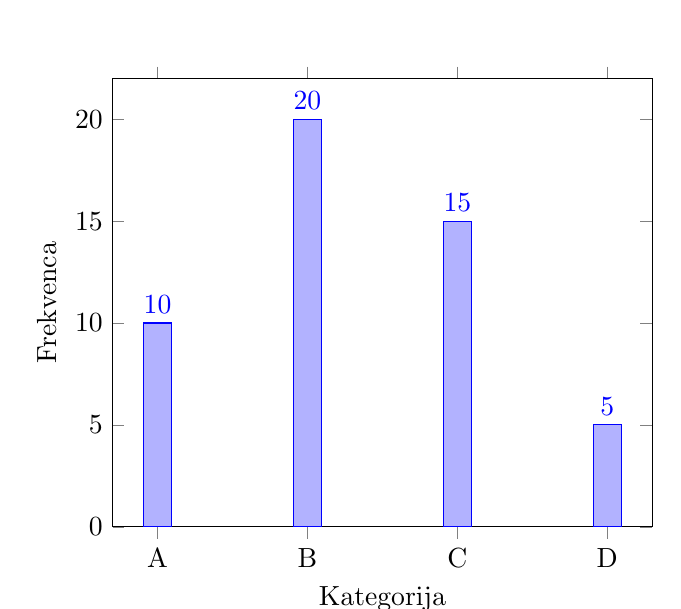
\begin{tikzpicture}
    \begin{axis}[
        ybar,
        symbolic x coords={A, B, C, D},
        xtick=data,
        ymin=0,
        ylabel={Frekvenca},
        xlabel={Kategorija},
        nodes near coords,
        ]
    \addplot coordinates {(A, 10) (B, 20) (C, 15) (D, 5)};
    \end{axis}
    \end{tikzpicture}
    \caption{Stolpčni grafikon frekvenc za nominalne spremenljivke.}
    \end{figure}

\section{Grafična predstavitev frelvenčnih porazdelitev za intervalne in razmernostne spremenljivke}

Histogram je vrsta stolpčnega grafikona, kjer stolpci predstavljajo frekvence podatkov v določenih intervalih. Histogram je uporaben za prikaz razpršenosti podatkov in za ugotavljanje oblik porazdelitev, kot so normalna, enakomerno porazdeljena ali pristranska porazdelitev.

\begin{figure}
    \centering
    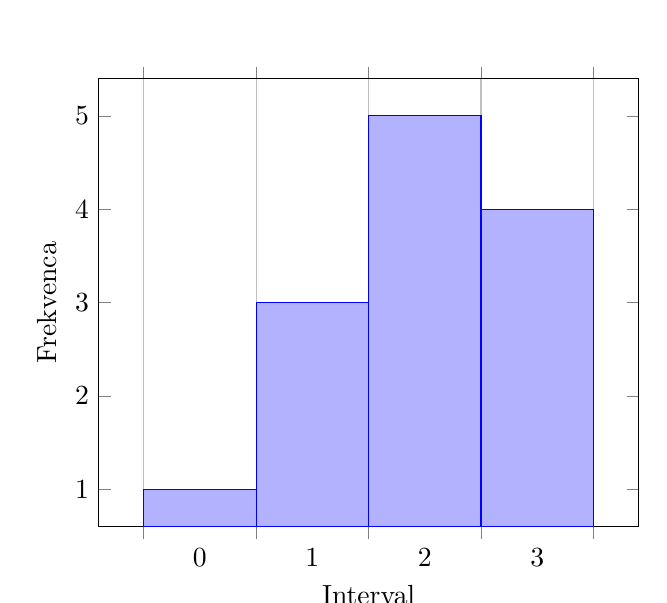
\begin{tikzpicture}
    \begin{axis}[
        ybar interval,
        ylabel={Frekvenca},
        xlabel={Interval},
        ]
    \addplot coordinates {(0, 1) (1, 3) (2, 5) (3, 4) (4, 2)};
    \end{axis}
    \end{tikzpicture}
    \caption{Histogram frekvenc za intervalne spremenljivke.}
\end{figure}

Poligon frekvenc je črtni grafikon, ki povezuje sosednje točke, ki predstavljajo frekvence intervalov. Uporablja se za prikaz porazdelitve podatkov in omogoča enostavno primerjavo z drugimi porazdelitvami.

\begin{figure}
    \centering
    \begin{tikzpicture}
    \begin{axis}[
        ylabel={Frekvenca},
        xlabel={Interval},
        ]
    \addplot coordinates {(0, 1) (1, 3) (2, 5) (3, 4) (4, 2)};
    \end{axis}
    \end{tikzpicture}
    \caption{Poligon frekvenc za intervalne spremenljivke.}
\end{figure}

Ogiva je črtni grafikon, ki prikazuje kumulativne frekvence. To pomeni, da vsaka točka na grafu predstavlja vsoto vseh prejšnjih frekvenc do določene vrednosti. Ogiva je uporabna za določanje percentilov in za primerjavo kumulativnih porazdelitev med različnimi skupinami podatkov.

\begin{figure}
    \centering
    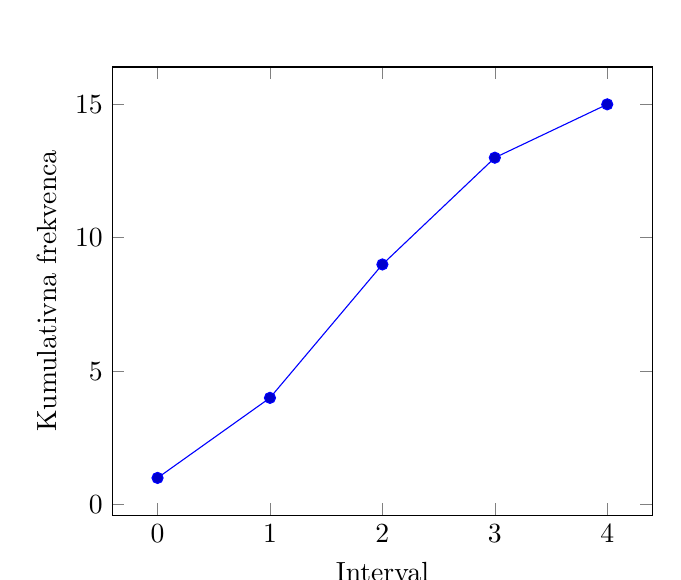
\begin{tikzpicture}
    \begin{axis}[
        ylabel={Kumulativna frekvenca},
        xlabel={Interval},
        ]
    \addplot coordinates {(0, 1) (1, 4) (2, 9) (3, 13) (4, 15)};
    \end{axis}
    \end{tikzpicture}
    \caption{Ogiva za kumulativne frekvence.}
\end{figure}

\section{Normalna porazdelitev}

Normalna porazdelitev je ena izmed najpomembnejših verjetnostnih porazdelitev v statistiki in se pogosto uporablja pri modeliranju različnih naravnih in družbenih pojavov. Gostotna funkcija normalne porazdelitve je podana z naslednjo enačbo:

\[f_X(x) = \frac{1}{\sigma\sqrt{2\pi}} e^{-\frac{1}{2} \frac{(x-\mu)^2}{\sigma^2}},\]

kjer je $\mu$ povprečje (aritmetična sredina) in $\sigma$ standardni odklon. Graf normalne porazdelitve je zvonaste oblike in simetričen glede na povprečje $\mu$.

\begin{figure}
\centering
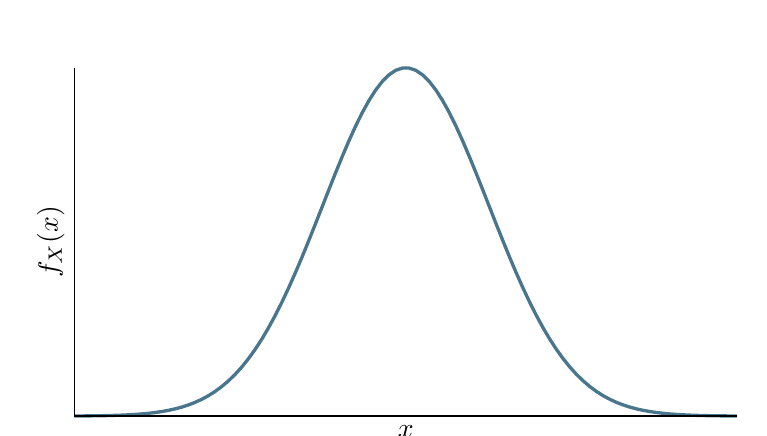
\begin{tikzpicture}
\begin{axis}[
    no markers, 
    domain=-4:4, 
    samples=100, 
    axis lines*=left, 
    xlabel=$x$, 
    ylabel=$f_X(x)$,
    height=6cm, 
    width=10cm, 
    xtick=\empty, 
    ytick=\empty,
    enlargelimits=false, 
    clip=false, 
    axis on top,
    grid = major
    ]
    \addplot[very thick,cyan!50!black] {1/(sqrt(2*pi))*exp(-x^2/2)};
\end{axis}
\end{tikzpicture}
\caption{Gostotna funkcija normalne porazdelitve.}
\end{figure}

\subsection{Asimetričnost (skewness)}

Asimetričnost meri, kako je porazdelitev nagnjena v levo ali desno. Normalna porazdelitev je popolnoma simetrična in ima koeficient asimetričnosti $k = 0$. Vendar pa v realnih podatkih pogosto srečamo porazdelitve, ki niso povsem simetrične:

\begin{itemize}
    \item Negativna asimetričnost (v levo, $k < 0$): Rep porazdelitve je daljši na levi strani.
    \item Pozitivna asimetričnost (v desno, $k > 0$): Rep porazdelitve je daljši na desni strani.
\end{itemize}

Če je $k$ med -1 in 1, se porazdelitev še vedno lahko šteje za normalno.

\begin{figure}
\centering
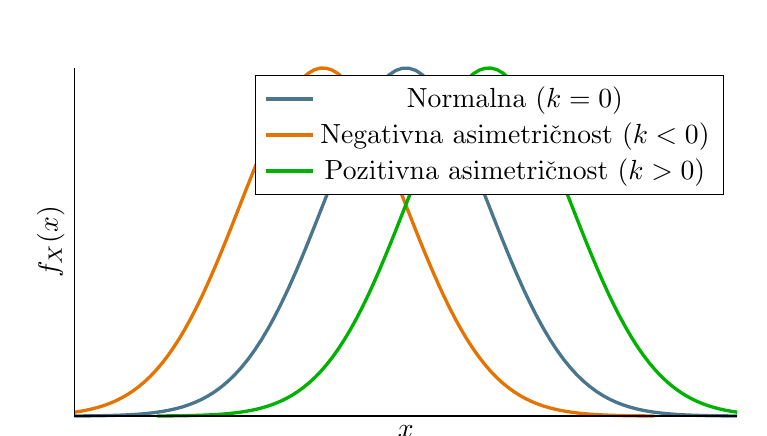
\begin{tikzpicture}
\begin{axis}[
    no markers, 
    domain=-4:4, 
    samples=100, 
    axis lines*=left, 
    xlabel=$x$, 
    ylabel=$f_X(x)$,
    height=6cm, 
    width=10cm, 
    xtick=\empty, 
    ytick=\empty,
    enlargelimits=false, 
    clip=false, 
    axis on top,
    grid = major
    ]
    \addplot[very thick,cyan!50!black] {1/(sqrt(2*pi))*exp(-x^2/2)};
    \addplot[very thick,orange!90!black, domain=-4:3] {1/(sqrt(2*pi))*exp(-((x+1)^2)/2)};
    \addplot[very thick,green!70!black, domain=-3:4] {1/(sqrt(2*pi))*exp(-((x-1)^2)/2)};
    \legend{Normalna ($k=0$), Negativna asimetričnost ($k<0$), Pozitivna asimetričnost ($k>0$)}
\end{axis}
\end{tikzpicture}
\caption{Grafi normalne porazdelitve s pozitivno in negativno asimetričnostjo.}
\end{figure}

\subsection{Sploščenost (kurtosis)}

Sploščenost meri, kako visoka in ostra je konica porazdelitve v primerjavi z normalno porazdelitvijo:

\begin{itemize}
    \item Leptokurtična ($k > 0$): Porazdelitev ima ožjo in višjo konico ter debelejše repe.
    \item Mezokurtična ($k = 0$): Porazdelitev je normalno zvonaste oblike.
    \item Platokurtična ($k < 0$): Porazdelitev ima ploščato konico in tanjše repe.
\end{itemize}

Če je $k$ med -1 in 1, se porazdelitev še vedno lahko šteje za normalno.

\begin{figure}
\centering
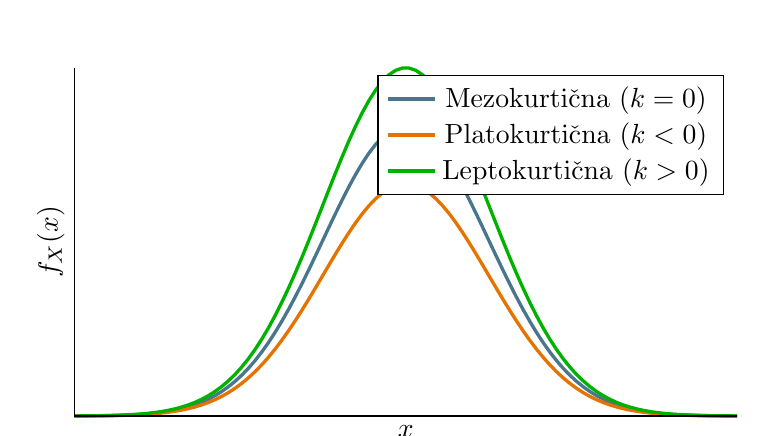
\begin{tikzpicture}
\begin{axis}[
    no markers, 
    domain=-4:4, 
    samples=100, 
    axis lines*=left, 
    xlabel=$x$, 
    ylabel=$f_X(x)$,
    height=6cm, 
    width=10cm, 
    xtick=\empty, 
    ytick=\empty,
    enlargelimits=false, 
    clip=false, 
    axis on top,
    grid = major
    ]
    \addplot[very thick,cyan!50!black] {1/(sqrt(2*pi))*exp(-x^2/2)};
    \addplot[very thick,orange!90!black] {0.8/(sqrt(2*pi))*exp(-x^2/2)};
    \addplot[very thick,green!70!black] {1.2/(sqrt(2*pi))*exp(-x^2/2)};
    \legend{Mezokurtična ($k=0$), Platokurtična ($k<0$), Leptokurtična ($k>0$)}
\end{axis}
\end{tikzpicture}
\caption{Grafi normalne porazdelitve s pozitivno in negativno sploščenostjo.}
\end{figure}

\section{Rangiranje}

Rangiranje vključuje razvrščanje podatkovnih točk v naraščajočem ali padajočem vrstnem redu. Rang določene vrednosti v podatkovnem naboru je njeno mesto v tem vrstnem redu. Rangiranje je uporabno za prepoznavanje relativnega položaja podatkovne točke znotraj nabora podatkov.

\textbf{Primer:}
\begin{itemize}
    \item Podatkovni niz: $45, 32, 67, 23, 89, 56$
    \item Urejeni podatkovni niz: $23, 32, 45, 56, 67, 89$
    \item Rangiranje: 
    \begin{itemize}
        \item 23 ima rang 1
        \item 32 ima rang 2
        \item 45 ima rang 3
        \item 56 ima rang 4
        \item 67 ima rang 5
        \item 89 ima rang 6
    \end{itemize}
\end{itemize}

\subsection{Kvantili}

Kvantili so vrednosti, ki delijo urejen niz podatkov na enake dele. Najpogosteje uporabljeni kvantili so kvartili, decili in percentili.

\textbf{Kvartili:}
Kvartili delijo podatkovni niz na štiri enake dele:
\begin{itemize}
    \item Prvi kvartil ($Q_1$): 25. percentil
    \item Drugi kvartil ($Q_2$): 50. percentil (median)
    \item Tretji kvartil ($Q_3$): 75. percentil
\end{itemize}

\textbf{Decili:}
Decili delijo podatkovni niz na deset enakih delov:
\begin{itemize}
    \item Prvi decil ($D_1$): 10. percentil
    \item Drugi decil ($D_2$): 20. percentil
    \item Tretji decil ($D_3$): 30. percentil
    \item itd.
\end{itemize}

\textbf{Percentili:}
Percentili delijo podatkovni niz na sto enakih delov:
\begin{itemize}
    \item 10. percentil: vrednost pod katero leži 10\% podatkov
    \item 50. percentil: vrednost pod katero leži 50\% podatkov (median)
    \item 90. percentil: vrednost pod katero leži 90\% podatkov
\end{itemize}

\textbf{Primer:}
Podatkovni niz: $15, 20, 35, 40, 50$
\begin{itemize}
    \item $Q_1$ (25. percentil): $20 + 0.25 \times (35 - 20) = 23.75$
    \item $Q_2$ (50. percentil): Median = $35$
    \item $Q_3$ (75. percentil): $35 + 0.75 \times (50 - 35) = 46.25$
\end{itemize}

\begin{figure}
\centering
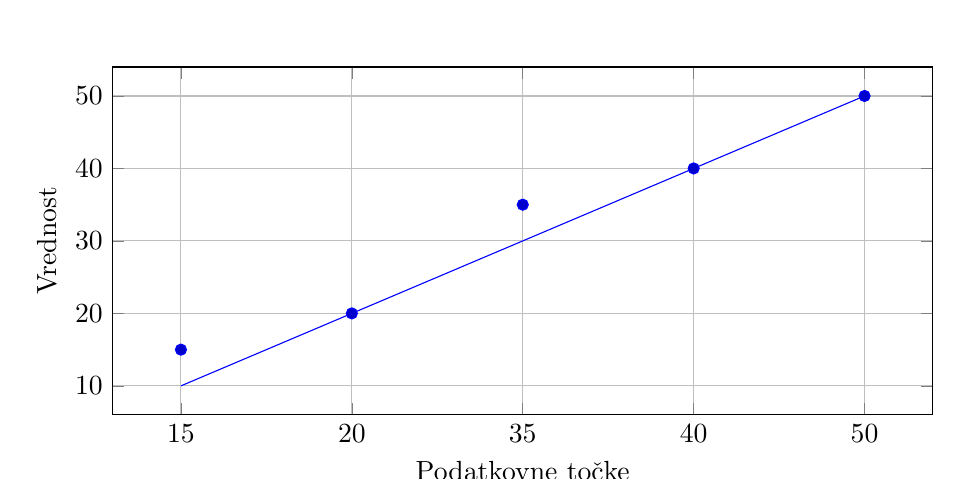
\begin{tikzpicture}
\begin{axis}[
    height=6cm,
    width=12cm,
    xtick={1, 2, 3, 4, 5},
    xticklabels={15, 20, 35, 40, 50},
    xlabel={Podatkovne točke},
    ylabel={Vrednost},
    ytick={0, 10, 20, 30, 40, 50, 60},
    grid=major
]
\addplot+[only marks,mark=*] coordinates {(1, 15) (2, 20) (3, 35) (4, 40) (5, 50)};
\addplot[domain=1:5, samples=5, color=blue] {x * 10};
\end{axis}
\end{tikzpicture}
\caption{Prikaz podatkovnega niza in kvantilov.}
\end{figure}

\section{Mere centralne tendence}
\begin{itemize}
    \item \textbf{Modus} - vrednost, ki se najpogosteje pojavi v nizu vrednosti podatkov
    \item \textbf{Mediana} - vrednost, ki ločuje zgornjo polovico obsega razpona vrednosti od spodnje polovice
    \item \textbf{Aritmetična sredina} - povprečje niza vrednosti
    \item Druge mere (geometrijska, harmonična sredina, ...)
\end{itemize}
Primerjava med modusom, mediano in aritmetično za unimodalne asimetrične - slika

\section{Mere variabilnosti (disperzije)}
V kolikšni meri se vrednosti razlikujejo med seboj ter razlikujejo in odstopajo od povprečja. Delimo jih na:
\begin{itemize}
    \item Absolutne mere (razpon, interkvartilni rang, absolutna deviacija aritmetične sredine/mediane, varianca in standardni odklon) 
    \item Relativne mere (absolutne mere deljene s pripadajočo mero centralne tendence) se izračunajo samo za razmernostne spremenljivke; uporabljamo jih, ko želimo primerjati:
    \begin{itemize}
        \item Dve porazdelitvi z zelo različno vrednostjo za nek mero centralne tendence;
        \item Dve spremenljivki z različnima merskima enotama.
    \end{itemize}
\end{itemize}

\subsection*{Razpon}

Absolutni razpon \[R_{abs}=x_{max}-x_{min}\]

Relativni razpon \[R_{rel}=\frac{2\left(x_{max}-x_{min}\right)}{x_{max}+x_{min}}\]

\subsection*{Interkvartilni rang}

\[IQR =\frac{Q_3 -Q_1}{2}\]

\subsection*{Absolutna deviacija mediane/aritmetične sredine}

\[AD_{Me,\mu}=\frac{1}{N}\sum_{i=1}^{N}|x_i - Me,\mu|\]

\subsection*{Varianca in standardni odklon}

\[\sigma^2 = \frac{1}{N} \sum_{i=1}^{N} (x_i - \mu)^2\]

\[\sigma = \sqrt{\sigma^2}\]

\subsection*{Variabilnost normalne porazdelitve}

Slika naslednjega

\begin{itemize}
    \item 68,3\% enot je znotraj enega standardnega odklona od povprečja \([\mu - \sigma, \mu + \sigma]\)
    \item 95,4\% enot je znotraj dveh standardnih odklonov od povprečja \([\mu - 2\sigma, \mu + 2\sigma]\)
    \item 99,7\% enot je znotraj treh standardnih odklonov od povprečja \([\mu - 3\sigma, \mu + 3\sigma]\)
\end{itemize}

\subsection*{Standardizacija}

\[z_i = \frac{x_i - \mu_X}{\sigma_X}\]

Rezultat je standardizirana spremenljivka $Z$, kjer standardizirane vrednosti $z_i$ predstavljajo relativna odstopanja od aritmetične sredine. Standardizacija nam omogoča primerjavo vrednosti različnih spremenljivk, ki praviloma niso primerljive.

Primer primerjave teže in višine dojenčkov, kjer standardiziramo glede na spol.

\begin{table}[h!]
    \centering
    \begin{tabular}{cccccc}
    \toprule
    Dojenček & Spol & Teža (kg) & $\mu_X$ (kg) & $\sigma_X$ (kg) & $z_i$ \\
    \midrule
    1 & Moški & 3.5 & 3.4 & 0.5 & $z_1 = \frac{3.5 - 3.4}{0.5} = 0.2$ \\
    2 & Ženski & 3.0 & 3.2 & 0.4 & $z_2 = \frac{3.0 - 3.2}{0.4} = -0.5$ \\
    3 & Moški & 4.0 & 3.4 & 0.5 & $z_3 = \frac{4.0 - 3.4}{0.5} = 1.2$ \\
    4 & Ženski & 2.8 & 3.2 & 0.4 & $z_4 = \frac{2.8 - 3.2}{0.4} = -1.0$ \\
    \bottomrule
    \end{tabular}
    \caption{Standardizacija teže dojenčkov glede na spol.}
\end{table}

\begin{Vaje}{1}
    Učence smo testirali v znanju matematike in dosegli so naslednje rezultate:
\[
\begin{array}{cccccccccccccc}
20 & 17 & 25 & 20 & 12 & 25 & 18 & 16 & 25 \\
17 & 21 & 22 & 22 & 16 & 17 & 22 & 20 & 19 & 16 \\
24 & 20 & 15 & 14 & 23 & 15 & 19 & 21 & 26 \\
18 & 29 & 30 & 20 & 16 & 12 & 24 & 30 & 27 & 25 \\
15 & 25 & 24 & 23 & 26 & 21 \\
\end{array}
\]

\begin{enumerate}
\item Poišči rezultat z rangom 8 (od najslabšega).
\item Koliko \% učencev je doseglo več kot 22 točk?
\item Kateri rezultat (ali rezultati) se najpogosteje pojavlja?
\item Rezultate testiranja razvrsti v frekvenčno porazdelitev.
\item Podatke prikaži grafično.
\end{enumerate}
\end{Vaje}

\begin{Vaje}{2} 
        Skupino desetih učencev smo testirali s psihodiagnostičnim testom in dobili naslednje rezultate:
        \[
        \begin{array}{cccccccccc}
        17 & 26 & 22 & 15 & 18 & 27 & 16 & 20 & 18 & 24 \\
        \end{array}
        \]
        
        \begin{enumerate}
            \item Izračunaj kvartile.
            \item Določi kvantilni rang vrednosti $x = 22.50$.
            \item Določi kvantilni rang rezultata $x = 22.00$.
        \end{enumerate}
\end{Vaje}

\begin{Vaje}{3}
    Na eni izmed avtošol smo se pozanimali, Koliko ur vožnje so kandidati potrebovali, preden so uspešno opravili vozniški izpit. Izračunaj aritmetično sredino, varianco in standardni odklon.
\end{Vaje}
\section{Inferenčna statistika}
\chapter{Bivariantna analiza}

\section{T-test}

\subsection{T-test za (parne) odvisne vzorce}

Primerjava povprečij dveh pogojev, v katerih so sodelovale iste enote.

Primer: 20 študentov je dobilo test v izpolnjevanje pred študijem določenega predmeta in nato ponovno po zaključku tega predmeta.

Testna statistika $t=\frac{\bar{d}}{SE(\bar{d})}$.

Izračun:

\begin{enumerate}
    \item Postavimo ničelno in alternativno hipotezo:
        \begin{itemize}
            \item $H_0$: Ni razlik v znanju študentov pred in po študiju tega modula.
            \item $H_1$: Obstajajo razlike v znanju študentov pred in po študiju tega modula.
        \end{itemize}
    \item Izračunamo razlike med pari opazovanj: $d_i = y_i - x_i$ (za vajo lahko to naredimo v SPSS).
    \item Izračunamo povprečje razlik: $\bar{d}$.
    \item Standardni odklon razlik: $s_d$.
    \item Standardna napaka povprečne razlike: $SE(\bar{d}) = \frac{s_d}{\sqrt{n}}$.
    \item T-statistika: $t = \frac{\bar{d}}{SE(\bar{d})}$ (empirična vrednost); $df = n-1$.
    \item V tabeli poiščemo kritično vrednost pri $\alpha = 5\%$.
    \item Empirična vrednost $t$ pade v kritično območje, ki ga določa teoretična vrednost $t$ pri dani stopnji zaupanja, zato lahko zavrnemo ničelno hipotezo in sprejmemo alternativno. Napiši kaj, če ne pade v kritično območje!
    \item Interval zaupanja za resnično vrednost razlike povprečij je: 
        \[\bar{d} \pm (t \cdot SE(\bar{d}))\]
\end{enumerate}

\subsection{T-test za neodvisne vzorce}

Primerjava preizkusa domneve o srednjih vrednosti dveh skupin enot.

Primer: Primerjava kalorične vrednosti dveh vrst štrudlja.

Testna statistika $t = \frac{\bar{x_1}-\bar{x_2}}{SE(\bar{x_1}-\bar{x_2})}$.

Opomba: Test predpostavi enakost varianc neodvisnih vzorcev. Če to ni zagotovoljeno, uporabimo Welchov test $t = \frac{\bar{x_1}-\bar{x_2}}{\sqrt{\frac{s_1^2}{n_1}+\frac{s_2^2}{n_2}}}$.

Izračun:
\begin{enumerate}
    \item Postavimo ničelno in alternativno hipotezo:
        \begin{itemize}
            \item $H_0$: Ni razlik v kalorični vsebnosti med dvema vrstama hotdoga.
            \item $H_1$: So razlike v kalorični vsebnosti med dvema vrstama hotdoga.
        \end{itemize}
    \item Razlika med povprečnima vrednostima: $\bar{x}_1 - \bar{x}_2$.
    \item Skupni standardni odklon (pod predpostavko enakih varianc):
        \[s_p = \sqrt{\frac{(n_1 - 1) \cdot s_1^2 + (n_2 - 1) \cdot s_2^2}{n_1 + n_2 - 2}}\]
    \item Standardna napaka: 
        \[SE(\bar{x}_1 - \bar{x}_2) = s_p \cdot \sqrt{\frac{1}{n_1} + \frac{1}{n_2}}\]
    \item Empirična t-vrednost: 
        \[t = \frac{\bar{x}_1 - \bar{x}_2}{SE(\bar{x}_1 - \bar{x}_2)}\]
    \item Prostostne stopnje: $df = n_1 + n_2 - 2$.
    \item V tabeli poiščemo kritično vrednost pri $\alpha = 5\%$.
    \item Interval zaupanja za resnično vrednost razlike povprečij: 
        \[\bar{x}_1 - \bar{x}_2 \pm (t \cdot SE(\bar{x}_1 - \bar{x}_2))\]
\end{enumerate}

\section{Analiza variance (ANOVA)}

Primerjava povprečij večih skupin (če sta samo dve skupini, je ANOVA enaka T testu).

$F$ porazdelitev ima dve prostorski skopnji.

\begin{figure}[h]
    \centering
    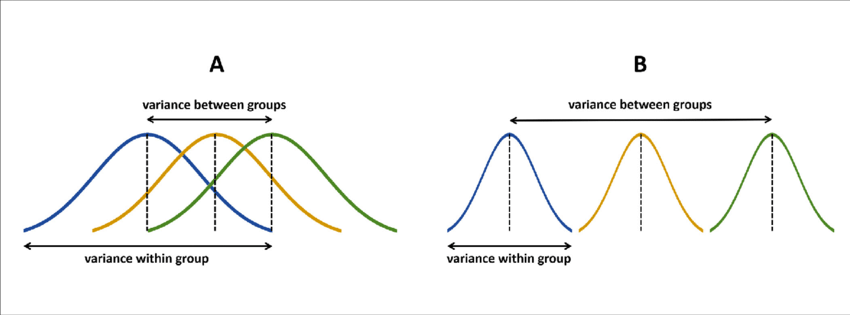
\includegraphics[width=\textwidth]{pictures/anova_varianca.png}
    \caption{This is a caption for the figure.}
    \label{fig:anova_varianca}
\end{figure}

Primer: Tri skupine desetih slučajno izbranih študentov so postavljene v tri različne učilnice. A ima konstantno glasbo v ozadju, B variabilno glasbo v ozadju, C brez glasbe. Po enem mesecu nas zanima, ali glasba pomaga pri učenju.

Izračun:
\begin{enumerate}
    \item Postavimo ničelno in alternativno hipotezo:
        \begin{itemize}
            \item $H_0$: Med skupinami ni razlik v vsrkavanju informacij.
            \item $H_1$: Med skupinami so razlike v vsrkavanju informacij.
        \end{itemize}
    \item Izračunamo povprečja. Skupno povprečje je $\bar{x} = 5,1$, povprečja posameznih skupin pa so $\bar{x}_1 = 7$, $\bar{x}_2 = 4$, in $\bar{x}_3 = 4,3$.
    \item Vsota kvadratov:
        \begin{itemize}
            \item Med skupinami: $SS_{between} = 54,6$
            \item Znotraj skupin: $SS_{within} = 90,1$
        \end{itemize}
    \item Prostostne stopnje:
        \begin{itemize}
            \item Med skupinami: $df_{between} = 2$
            \item Znotraj skupin: $df_{within} = 27$
        \end{itemize}
    \item Povprečni kvadrat:
        \begin{itemize}
            \item Med skupinami: $MS_{between} = \frac{SS_{between}}{df_{between}} = \frac{54,6}{2} = 27,3$
            \item Znotraj skupin: $MS_{within} = \frac{SS_{within}}{df_{within}} = \frac{90,1}{27} = 3,34$
        \end{itemize}
    \item Empirična F-vrednost: 
        \[F = \frac{MS_{between}}{MS_{within}} = \frac{27,3}{3,34} = 8,18\]
    \item V tabeli poiščemo kritično vrednost pri $\alpha = 5\%$: $F_{critical} = 2,03$.
    \item Ker je empirična F-vrednost (8,18) večja od kritične vrednosti (2,03), zavrnemo ničelno hipotezo $H_0$.
    \item Izračunamo eta kvadrat ($\eta^2$), ki je merilo učinka:
        \[\eta^2 = \frac{SS_{between}}{SS_{between} + SS_{within}} = \frac{54,6}{54,6 + 90,1} = 0,38\]
        \[ \eta = \sqrt{\eta^2} = \sqrt{0,38} \approx 0,62\]
\end{enumerate}

\section{Neparametrične alternative}

Če podatki niso normalno porazdeljeni, moramo parametrični test zamenjati z ustreznim neparametričnim testom.

\begin{table}[h!]
    \centering
    \begin{tabular}{|l|l|l|}
    \hline
    \textbf{Cilj} & \textbf{Parametrični test} & \textbf{Neparametrični test} \\ \hline
    Testiranje razlike med dvema odvisnima nizoma enot & Odvisni $t$-test & Wilcoxon test predznačenih rangov \\ \hline
    Testiranje razlike med dvema neodvisnima nizoma enot & Neodvisni $t$-test & Mann-Whitney $U$ test \\ \hline
    Testiranje razlike med tremi ali več neodvisnimi nizi enot & ANOVA & Kruskal-Wallis $H$ test \\ \hline
    \end{tabular}
    \caption{Pregled parametričnih in neparametričnih testov}
\end{table}

\subsection{Hi-kvadrat test}

Uporablja se za ugotavljanje, ali obstaja statistično značilna razlika med pričakovanimi in opazovanimi frekvencami v eni ali več kategorijah (torej če imamo nomilane spremenljivke)

Ničelna hipoteza $H_0$: V populaciji ni povezanosti med spremenljivkama.

Slika hi kvadrat porazdelitve

\paragraph{Izračunavanje stopnje prostosti ($df$):}
Stopnja prostosti ($df$) za hi-kvadrat test se izračuna po formuli:
\[df = (\text{vrstice} - 1) \cdot (\text{stolpci} - 1)\]

\paragraph{Postopek izračuna:}
\begin{enumerate}
    \item Zberemo podatke in uredimo frekvence v kontingenčni tabeli.
    \item Izračunamo pričakovane frekvence za vsako celico tabele.
    \item Uporabimo formulo za hi-kvadrat vrednost:
    \[\chi^2 = \sum \frac{(O_i - E_i)^2}{E_i}\]
    kjer je $O_i$ opazovana frekvenca, $E_i$ pa pričakovana frekvenca.
\end{enumerate}

\paragraph{Uporaba kontingenčnih koeficientov:}
Ker vrednosti hi-kvadrat same po sebi niso primerljive med različnimi tabelami, pogosto uporabimo kontingenčne koeficiente, kot je Cramérjev $V$, ki ga izračunamo po formuli:
\[V = \sqrt{\frac{\chi^2}{N \cdot (k - 1)}},\]
kjer je $\chi^2$ hi-kvadrat vrednost, $N$ skupno število opazovanj, $k$ pa število kategorij v najbolj številni spremenljivki.

\subsection{Spearmanov koeficient}

Spearmanov koeficient korelacije meri moč in smer monotone povezave med dvema spremenljivkama. Uporablja se za ordinalne spremenljivke ali za kvantitativne spremenljivke, ki niso nujno normalno porazdeljene.

\paragraph{Ničelna hipoteza $H_0$:}
Med dvema spremenljivkama ni monotone povezave.

\paragraph{Formula:}
Spearmanov koeficient ($\rho$) se izračuna po formuli:
\[\rho = 1 - \frac{6 \sum d_i^2}{n(n^2 - 1)},\]
kjer je $d_i$ razlika med vrstnimi številkami vsakega opazovanja in $n$ število opazovanj.

\paragraph{Postopek izračuna:}
\begin{enumerate}
    \item Razvrstimo podatke v naraščajočem vrstnem redu za vsako spremenljivko.
    \item Izračunamo vrstne številke za vsako spremenljivko.
    \item Izračunamo razlike med vrstnimi številkami ($d_i$) za vsako opazovanje.
    \item Uporabimo zgornjo formulo za izračun Spearmanovega koeficienta.
\end{enumerate}

\paragraph{Interpretacija:}
Spearmanov koeficient se giblje med -1 in 1. Vrednost blizu 1 kaže na močno pozitivno monotono povezavo, vrednost blizu -1 kaže na močno negativno monotono povezavo, vrednost blizu 0 pa kaže na odsotnost monotone povezave.

\paragraph{Zaključek:}
Spearmanov koeficient je uporaben za analizo povezav med ordinalnimi ali kvantitativnimi spremenljivkami, ki niso normalno porazdeljene. Pomaga nam razumeti moč in smer monotone povezave med spremenljivkami.

\subsection{Pearsonov koeficient}

Pearsonov koeficient korelacije meri linearno povezanost med dvema kvantitativnima spremenljivkama. Uporablja se za intervalne ali razmerne spremenljivke, ki so normalno porazdeljene.

\paragraph{Ničelna hipoteza $H_0$:}
Med dvema spremenljivkama ni linearne povezave.

\paragraph{Formula:}
Pearsonov koeficient ($r$) se izračuna po formuli:
\[r = \frac{\sum (x_i - \bar{x})(y_i - \bar{y})}{\sqrt{\sum (x_i - \bar{x})^2 \sum (y_i - \bar{y})^2}},\]
kjer je $x_i$ in $y_i$ vsaka opazovanja za spremenljivki $x$ in $y$, $\bar{x}$ in $\bar{y}$ pa povprečji za spremenljivki $x$ in $y$.

\paragraph{Postopek izračuna:}
\begin{enumerate}
    \item Izračunamo povprečje za vsako spremenljivko.
    \item Izračunamo odstopanja vsakega opazovanja od povprečja.
    \item Pomnožimo odstopanja za ustrezna opazovanja in izračunamo vsoto.
    \item Izračunamo kvadrate odstopanj za vsako spremenljivko in vsoto kvadratov.
    \item Uporabimo zgornjo formulo za izračun Pearsonovega koeficienta.
\end{enumerate}

\paragraph{Interpretacija:}
Pearsonov koeficient se giblje med -1 in 1. Vrednost blizu 1 kaže na močno pozitivno linearno povezavo, vrednost blizu -1 kaže na močno negativno linearno povezavo, vrednost blizu 0 pa kaže na odsotnost linearne povezave.

\section{Povezanost}

Povezanost med dvema spremenljivkama pomeni, da spremembe v eni spremenljivki sovpadajo s spremembami v drugi spremenljivki. Povezanost lahko merimo na različne načine, odvisno od narave spremenljivk in vrste povezave.

\subsection*{Funkcionalna povezanost}
Funkcionalna povezanost pomeni, da obstaja točno določena matematična funkcija, ki povezuje dve spremenljivki. Na primer, če $y = f(x)$, potem je $y$ popolnoma določeno s $x$. To je najmočnejša oblika povezanosti, saj vsaka vrednost ene spremenljivke določa točno eno vrednost druge spremenljivke.

\subsection*{Korelacijska povezanost}
Korelacijska povezanost meri stopnjo in smer linearne povezave med dvema kvantitativnima spremenljivkama. Najpogosteje uporabljamo Pearsonov koeficient korelacije ($r$), ki meri linearno povezanost, in Spearmanov koeficient korelacije ($\rho$), ki meri monotono povezanost.

\subsection*{Močna in šibka povezanost}
Moč povezanosti se nanaša na velikost koeficienta korelacije. 
\begin{itemize}
    \item \textbf{Močna povezanost}: Koeficient korelacije blizu 1 ali -1 kaže na močno povezanost.
    \item \textbf{Šibka povezanost}: Koeficient korelacije blizu 0 kaže na šibko povezanost.
\end{itemize}

\subsection*{Linearna in nelinearna povezanost}
\begin{itemize}
    \item \textbf{Linearna povezanost}: Povezanost, kjer lahko povezavo med spremenljivkama najbolje opišemo z ravno črto. Pearsonov koeficient korelacije ($r$) je primeren za merjenje linearne povezanosti.
    \item \textbf{Nelinearna povezanost}: Povezanost, kjer je povezava med spremenljivkama bolj zapletena in je ni mogoče opisati z ravno črto. Spearmanov koeficient korelacije ($\rho$) je primeren za merjenje monotone (nelinearne) povezanosti.
\end{itemize}

\subsection*{Pozitivna in negativna povezanost}
\begin{itemize}
    \item \textbf{Pozitivna povezanost}: Ko se ena spremenljivka povečuje, se druga spremenljivka tudi povečuje. Koeficient korelacije je pozitiven.
    \item \textbf{Negativna povezanost}: Ko se ena spremenljivka povečuje, se druga spremenljivka zmanjšuje. Koeficient korelacije je negativen.
\end{itemize}

\subsection{Kovarianca}

Kovarianca je mera, ki opisuje, kako se dve spremenljivki sočasno spreminjata. Pozitivna kovarianca pomeni, da se večje vrednosti ene spremenljivke povezujejo z večjimi vrednostmi druge spremenljivke, medtem ko negativna kovarianca pomeni, da se večje vrednosti ene spremenljivke povezujejo z manjšimi vrednostmi druge spremenljivke.

\paragraph{Formula}
Kovarianca dveh spremenljivk $X$ in $Y$ se izračuna po formuli:
\[\text{Cov}(X, Y) = \frac{1}{n-1} \sum_{i=1}^n (X_i - \bar{X})(Y_i - \bar{Y}),\]
kjer:
\begin{itemize}
    \item $X_i$ in $Y_i$ sta posamezni opazovanji spremenljivk $X$ in $Y$,
    \item $\bar{X}$ in $\bar{Y}$ sta povprečji spremenljivk $X$ in $Y$,
    \item $n$ je število opazovanj.
\end{itemize}

\paragraph{Interpretacija}
\begin{itemize}
    \item \textbf{Pozitivna kovarianca}: Ko se vrednosti ene spremenljivke povečujejo, se povečujejo tudi vrednosti druge spremenljivke.
    \item \textbf{Negativna kovarianca}: Ko se vrednosti ene spremenljivke povečujejo, se vrednosti druge spremenljivke zmanjšujejo.
    \item \textbf{Kovarianca blizu nič}: Ni jasno izražene povezave med spremenljivkama.
\end{itemize}

\paragraph{Razlika med kovarianco in korelacijo}

Kovarianca meri le smer sočasnih sprememb dveh spremenljivk, vendar ni standardizirana, zato njena vrednost ni omejena. Po drugi strani pa je korelacija standardizirana mera, ki pove, kako močna in v katero smer je linearna povezava med dvema spremenljivkama, njena vrednost pa je vedno med -1 in 1.

\begin{Vaje}{1}
    V datoteki \href{https://github.com/borbregant/ai_tandem_learning/blob/main/data_cleaned.xlsx}{data\_cleaned.xlsx} določi naslednje:
    \begin{itemize}
        \item Ali obstaja povezava med matematično anksioznostjo in motivacijo za matematiko? Če je povezava znatna, določi še enačbo linearne regresije, kjer si sam izbereš odvisno in neodvisno spremenljivko.
        \item Ali obstaja povezava med spolom in anksioznostjo?
        \item Ali obstaja povezava med profesorjem in razredom?
    \end{itemize}
    Imej v mislih, da so kategorične spremenljivke v dokumentu kodirane označevalno.
\end{Vaje}

\section{Multivariantna statistika}



\begin{Vaje}{1}
    ...
\end{Vaje}


\end{document}